\documentclass[20pt, a0paper, portrait]{tikzposter}

\usepackage[utf8]{inputenc}
\usepackage[T1]{fontenc}
\renewcommand*\familydefault{\sfdefault}
\usepackage{textcomp}
\usepackage{arev}
\usepackage{arevmath}
\usepackage{arevtext}
\usepackage{graphicx}
\usepackage{wrapfig}
\usepackage{microtype}
\usepackage{subfig}

% Bibliography
\usepackage[backend=biber,
bibencoding=utf8,
bibstyle=numeric-comp,
%style=verbose, %verbose-ibid,
url=true, % include url in reference
doi=true, % include doi in reference
sorting=none, % sorting of citations
%autocite=superscript, % autocite becomes superscript
maxcitenames=1, % Max names displayed when citing in text
maxbibnames=10, % Max number of names displayed in the bibliography
giveninits=true % Use initials
]{biblatex}
\addbibresource{citations.bib}
\renewcommand*{\bibfont}{\footnotesize}

\title{Concept Generation}
\author{Engineering Design \& Manufacture Group}
\date{\today}
\institute{University of Bath, UK}

\usetheme{Default}
\usecolorstyle[colorPalette=GreenGrayViolet]{Default}
\useblockstyle{Default}
\usetitlestyle{Filled}

\begin{document}

\maketitle

\begin{columns}
  \column{0.5}
  \block[]{Introduction}{
    Concept generation is a fundamental part of any Engineering Design process. In this section, we discuss four methods that can be used in generating concepts.

    \vspace{1em}

    \begin{enumerate}
      \itemsep0cm
      \item Brainstorming
      \item Competitor analysis \& patent search
      \item Morphological charts
      \item Prototyping \& construction kits
    \end{enumerate}
  }
  \block[]{Brainstorming}{
    Brainstorming is a technique by which a group attempts to find a solution for a specific problem by amassing all the members' ideas spontaneously. Although many consider brainstorming as an ad-hoc exercise where teams get together to form ideas, rules and guidelines to maximise the creative output have been developed.

    \vspace{1em}

    Alex Osborn was one of the first to develop a rule-set for brainstorming. The objective was to improve the creation of new ideas within business meetings. The rules can be summarised as:

    \vspace{1em}

    \begin{itemize}
      \itemsep0cm
      \item No criticism of ideas
      \item Go for large quantities of ideas
      \item Build on other ideas or combine them
      \item Encourage wild and unusual ideas
    \end{itemize}

    \vspace{1em}

    Through these rules, his studies revealed that more ideas were created and \emph{``quantity produced quality''}.

    \vspace{1em}

    Since then, there have been many more studies into brainstorming and methods that can support the generation of ideas. Here are a just a few of them (Figure~\ref{fig-brainstorm}).

    \begin{tikzfigure}[Brainstorming techniques]
      \centering
      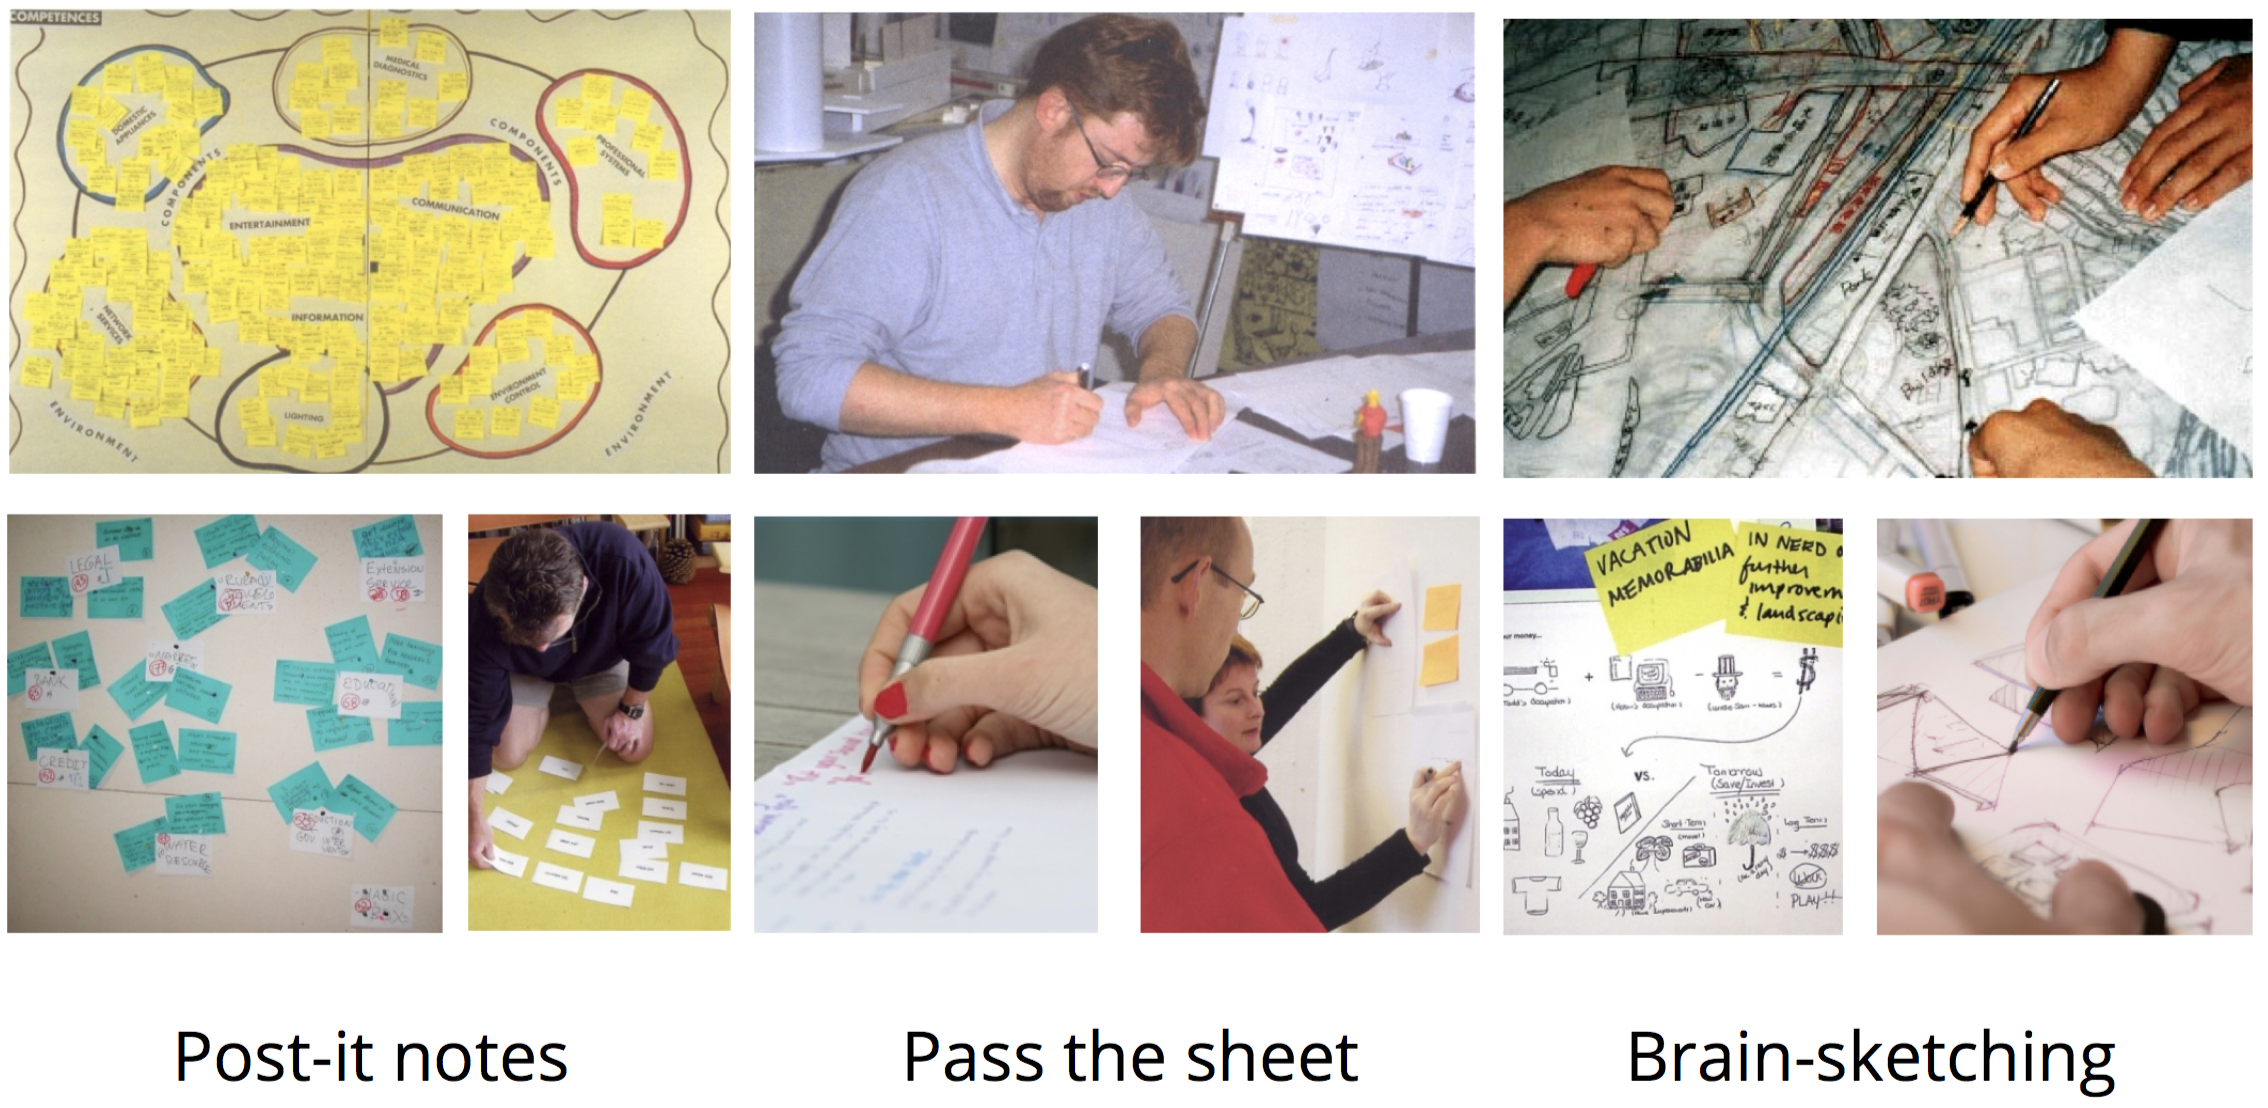
\includegraphics[width=0.4\textwidth]{figures/brainstorm.png}
      \label{fig-brainstorm}
    \end{tikzfigure}
    
    \textbf{Post-It Notes} The `Post-it Note' exercise requires engineers to write and/or sketch onto a post-it note. This is then placed on the table for the rest of the group to see. As more notes are added, the facilitator can start to form groups of notes that follow a similar theme and/or answer a particular part of the design task.

    \vspace{1em}
    
    \textbf{Pass the Sheet} In the `Pass the Sheet' exercise, each designer is given a sheet of paper and are asked to write a couple of sentences for a potential idea to solve the problem. These are then passed around to the next designer in the group who tries to build-upon the existing idea by writing an additional couple of sentences. Once passed around the whole group, the ideas are read aloud and a discussion is had on the relative merits from each one. The group then converges upon one of the ideas and/or combine features of each to develop their final concepts.

    \vspace{1em}
    
    \textbf{Brain-sketching} In `Brain-sketching', the group is not aloud to talk or write their ideas. All they can do is sketch. Annotations on the sketches may be permitted to convey what the item is. This is a great way of tackling challenges where form and/or packaging is a critical issue. 

  }
  \block[]{Competitor Analysis \& Patent Search}{
    More often than not, you will be developing a product that will be competing with and/or complementing an existing product line. Therefore, it is always a good idea to analyse existing products on the market with respect to your PDS.  Patent searching also enables you to discover what attempts have been made to solve the problem and what aspects might be protected by people across the world.

    \vspace{1em}

    The main advantages are that you will have confidence that a variation of an existing design has a greater potential to work when compared to a completely novel design. It also enables you to quickly generate potential designs. By comparing existing products to your PDS, you can start to identify areas that will make your product unique and help you decide where to focus your design resources and time on.

    \vspace{1em}

    The potential issue in using existing products is that you have the potential to infringe on intellectual property and copyright. The companies you will be working for will have legal teams to help you in deciding what elements of existing designs can be used.
  }
  \column{0.5}
  \block[]{Morphological Charts}{

    Morphological charts are a great method for generating ideas where the product to be designed has clear functional and/or sub-system boundaries. For each function, designers can come up with a range of potential solutions. From this, a matrix of function vs.\ solution can be created. An example is shown in Figure~\ref{fig-morphological-chart}.

    \begin{tikzfigure}[Morphological Chart]
      \centering
      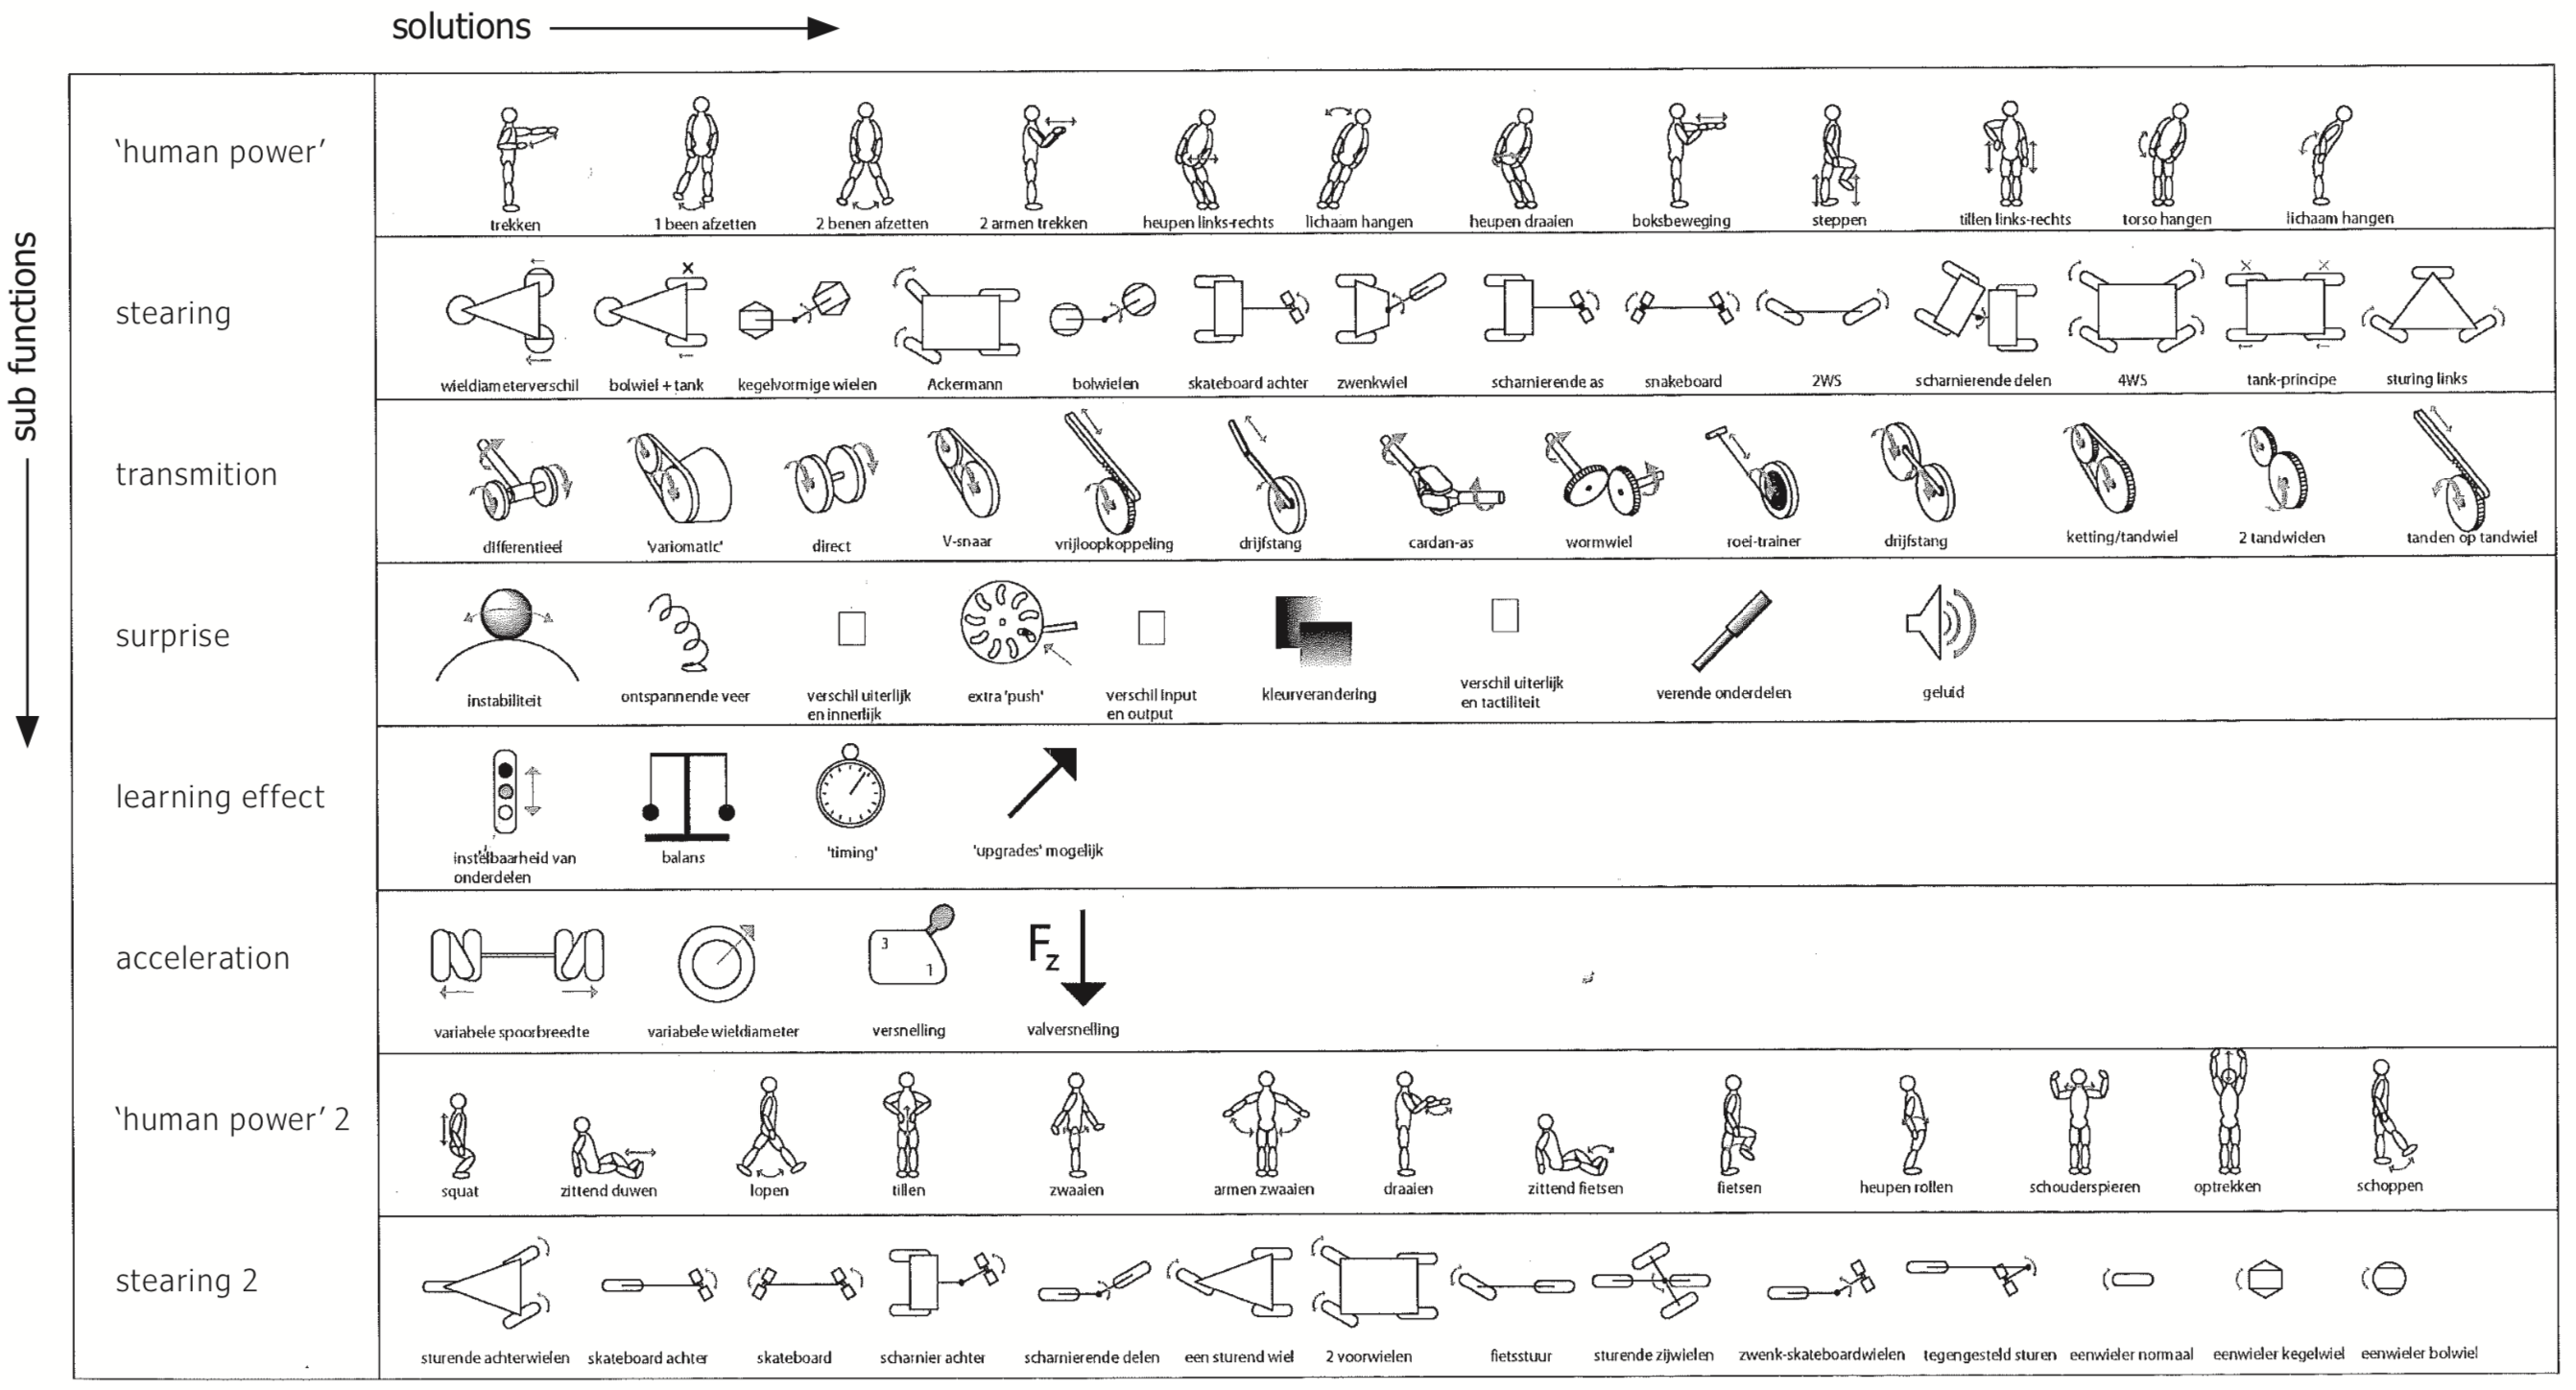
\includegraphics[width=0.4\textwidth]{figures/morphological-chart.png}
      \label{fig-morphological-chart}
    \end{tikzfigure}
  }
  \block[]{Prototyping \& Construction Kits}{

    Prototyping \& construction kits are a great way of quickly refining and identifying potential geometric issues during the early design phases (Figure~\ref{fig-why-prototype}). The use of kits such as LEGO\texttrademark{} remove the potential bias introduced by the quality of designers' sketches and wording of ideas as all ideas are created to the same level of refinement. The simplicity of these kits also enables wider stakeholder engagement where you can have you customers and different departments involved in the generation of potential solutions. In some instances, the design problem can be very large with multiple dependencies between requirements. Prototyping is a method that can focus the designers attention to specific parts of the design problem, which can then be later combined to form an overall concept (Figure~\ref{fig-why-prototype}).

    \begin{tikzfigure}[Bill Buxton, Sketching User Experiences~\autocite{buxton2010}]
    \centering
    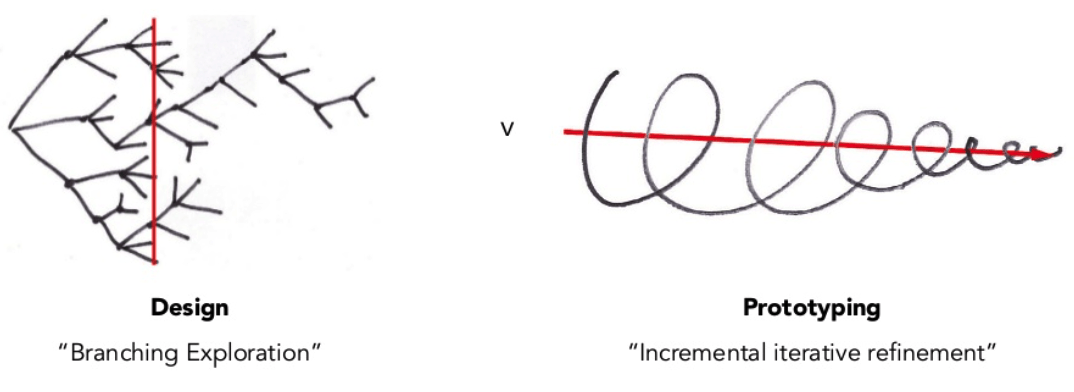
\includegraphics[width=0.4\textwidth]{figures/whyprototype.png}
    \label{fig-why-prototype}
    \end{tikzfigure}
    
    \textbf{Research at Bath} However, the use of prototyping and construction kits can introduce constraints and biases in the exploration of the potential solution space. For example, lets take 7 $2\times2$ LEGO\texttrademark{} bricks ($B_{2,2}(7)$), which we want to connect together by adding one brick at a time. In this scenario, there are 1.8e9 unique pathways of constructing the bricks and 1.3e6 morphologically unique combinations. The greater number of paths to unique combinations provide the perception that there are a lot more potential solutions than there actually are. Further, if one were to look at the number of pathways to each unique combination, some have more pathways than others and hence, are statistically more likely to be created by a designer. An example of this is shown in Figure~\ref{fig-combinations} and is part of the ongoing research at Bath where the findings are being used to help design future construction kits to support concept generation~\autocite{design2018}.

    \begin{tikzfigure}[$B_{2,2}(2)$ combinations]
      \centering
      \\
      \begin{tabular}{c c c}
        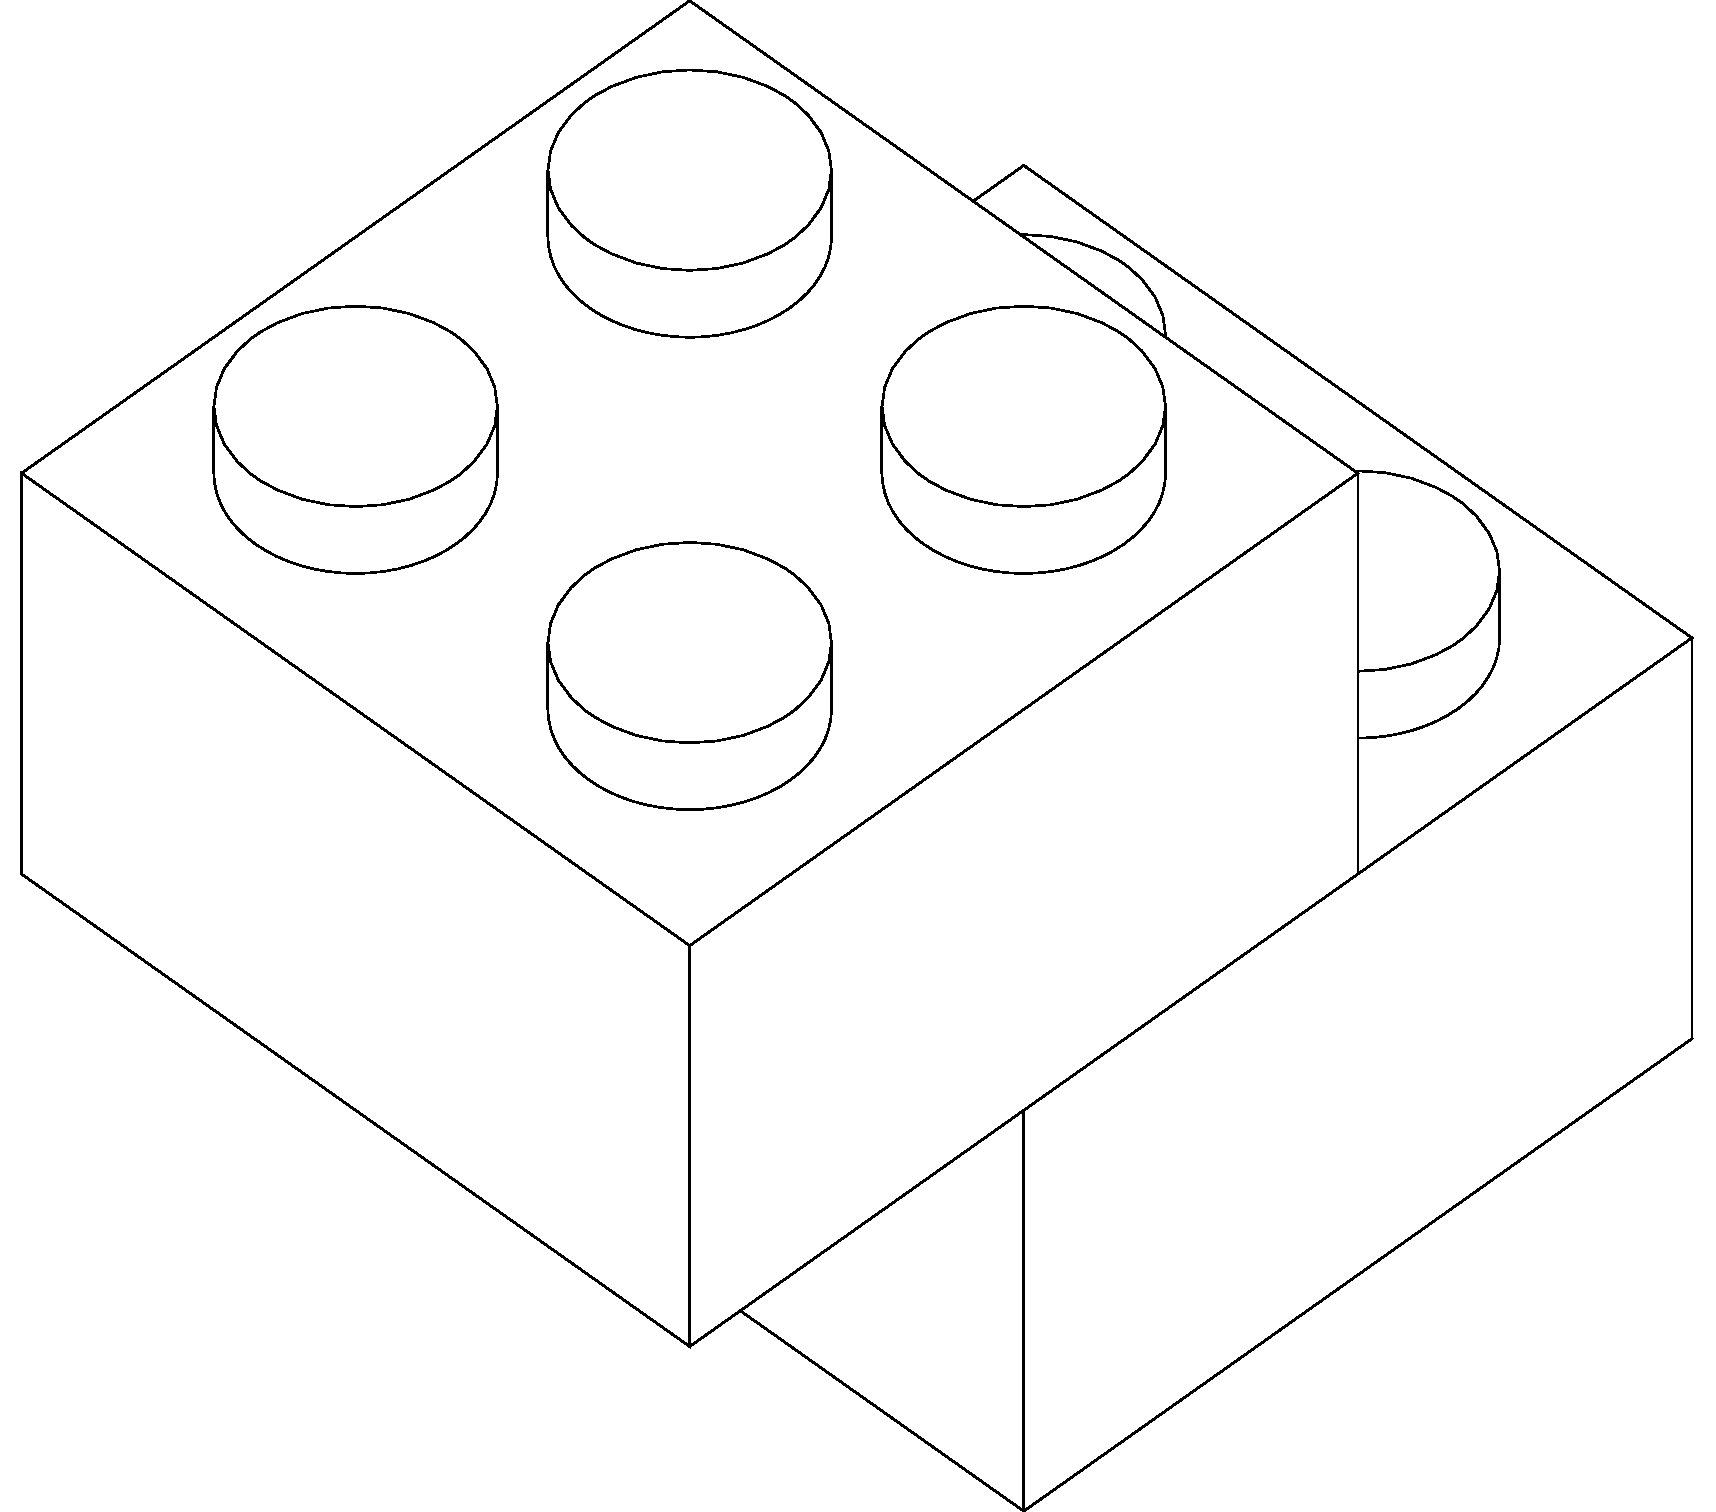
\includegraphics[width=0.12\textwidth]{figures/2x2-brick-combo-1.pdf}
        &
        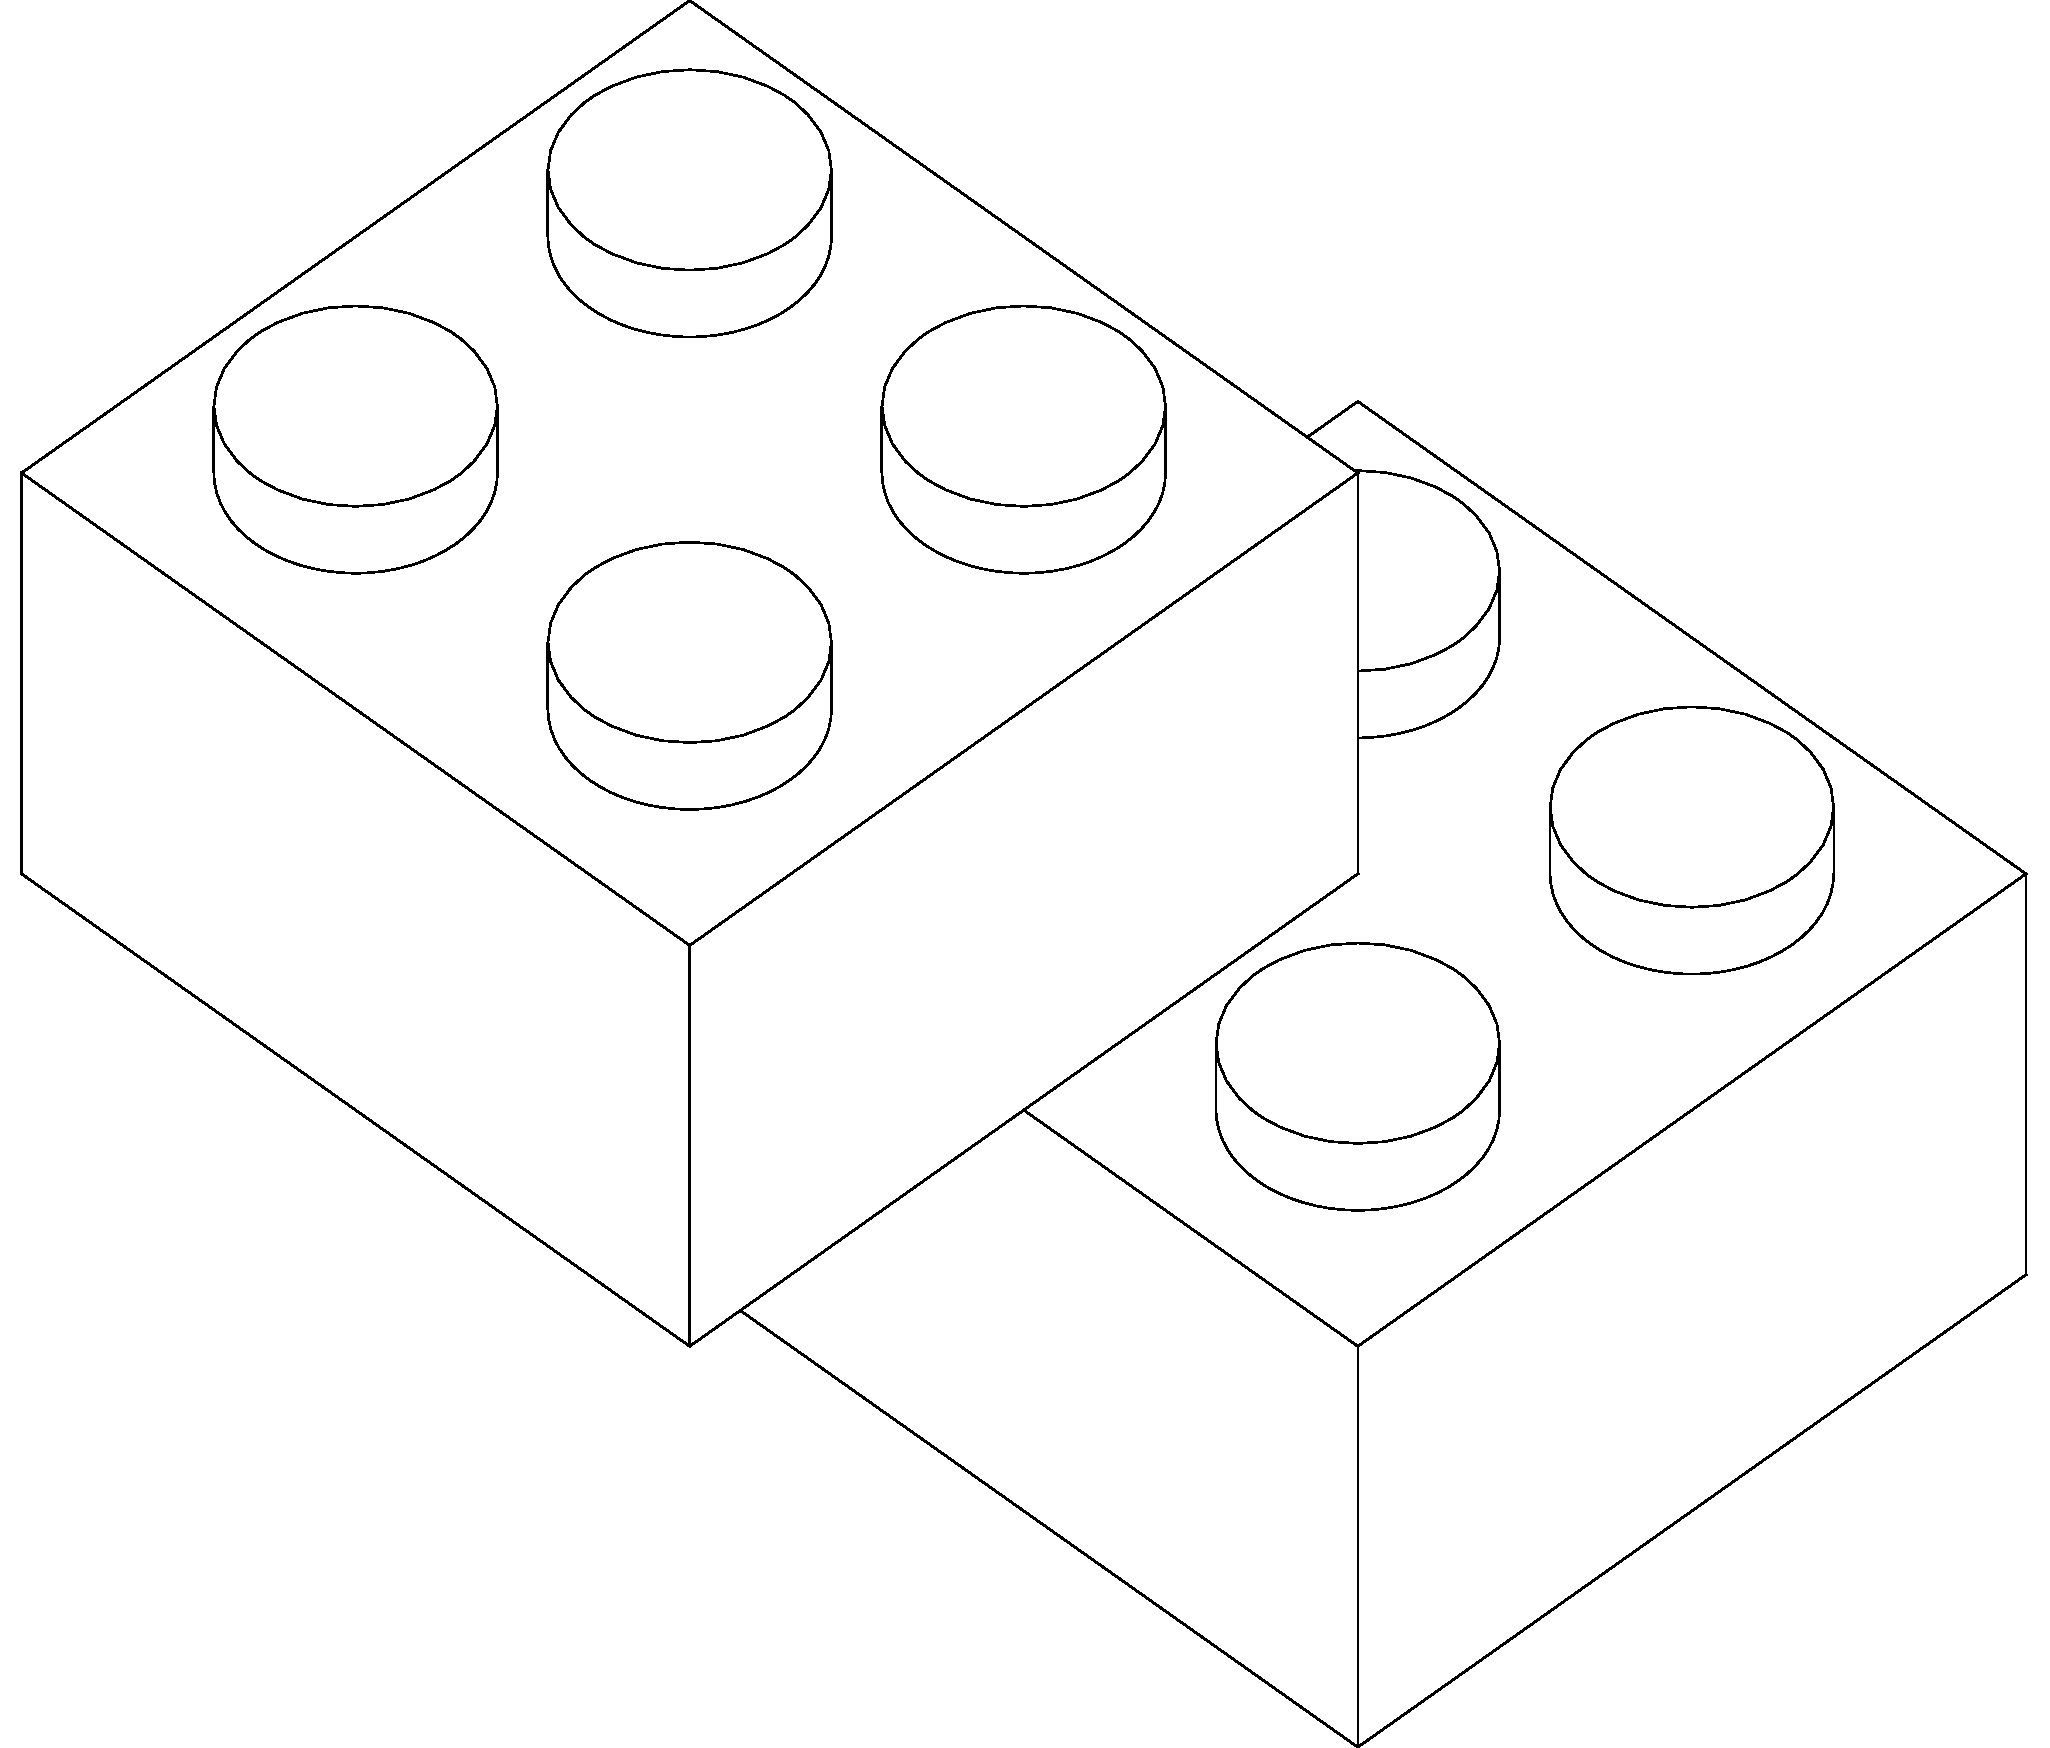
\includegraphics[width=0.13\textwidth]{figures/2x2-brick-combo-2.pdf}
        &
        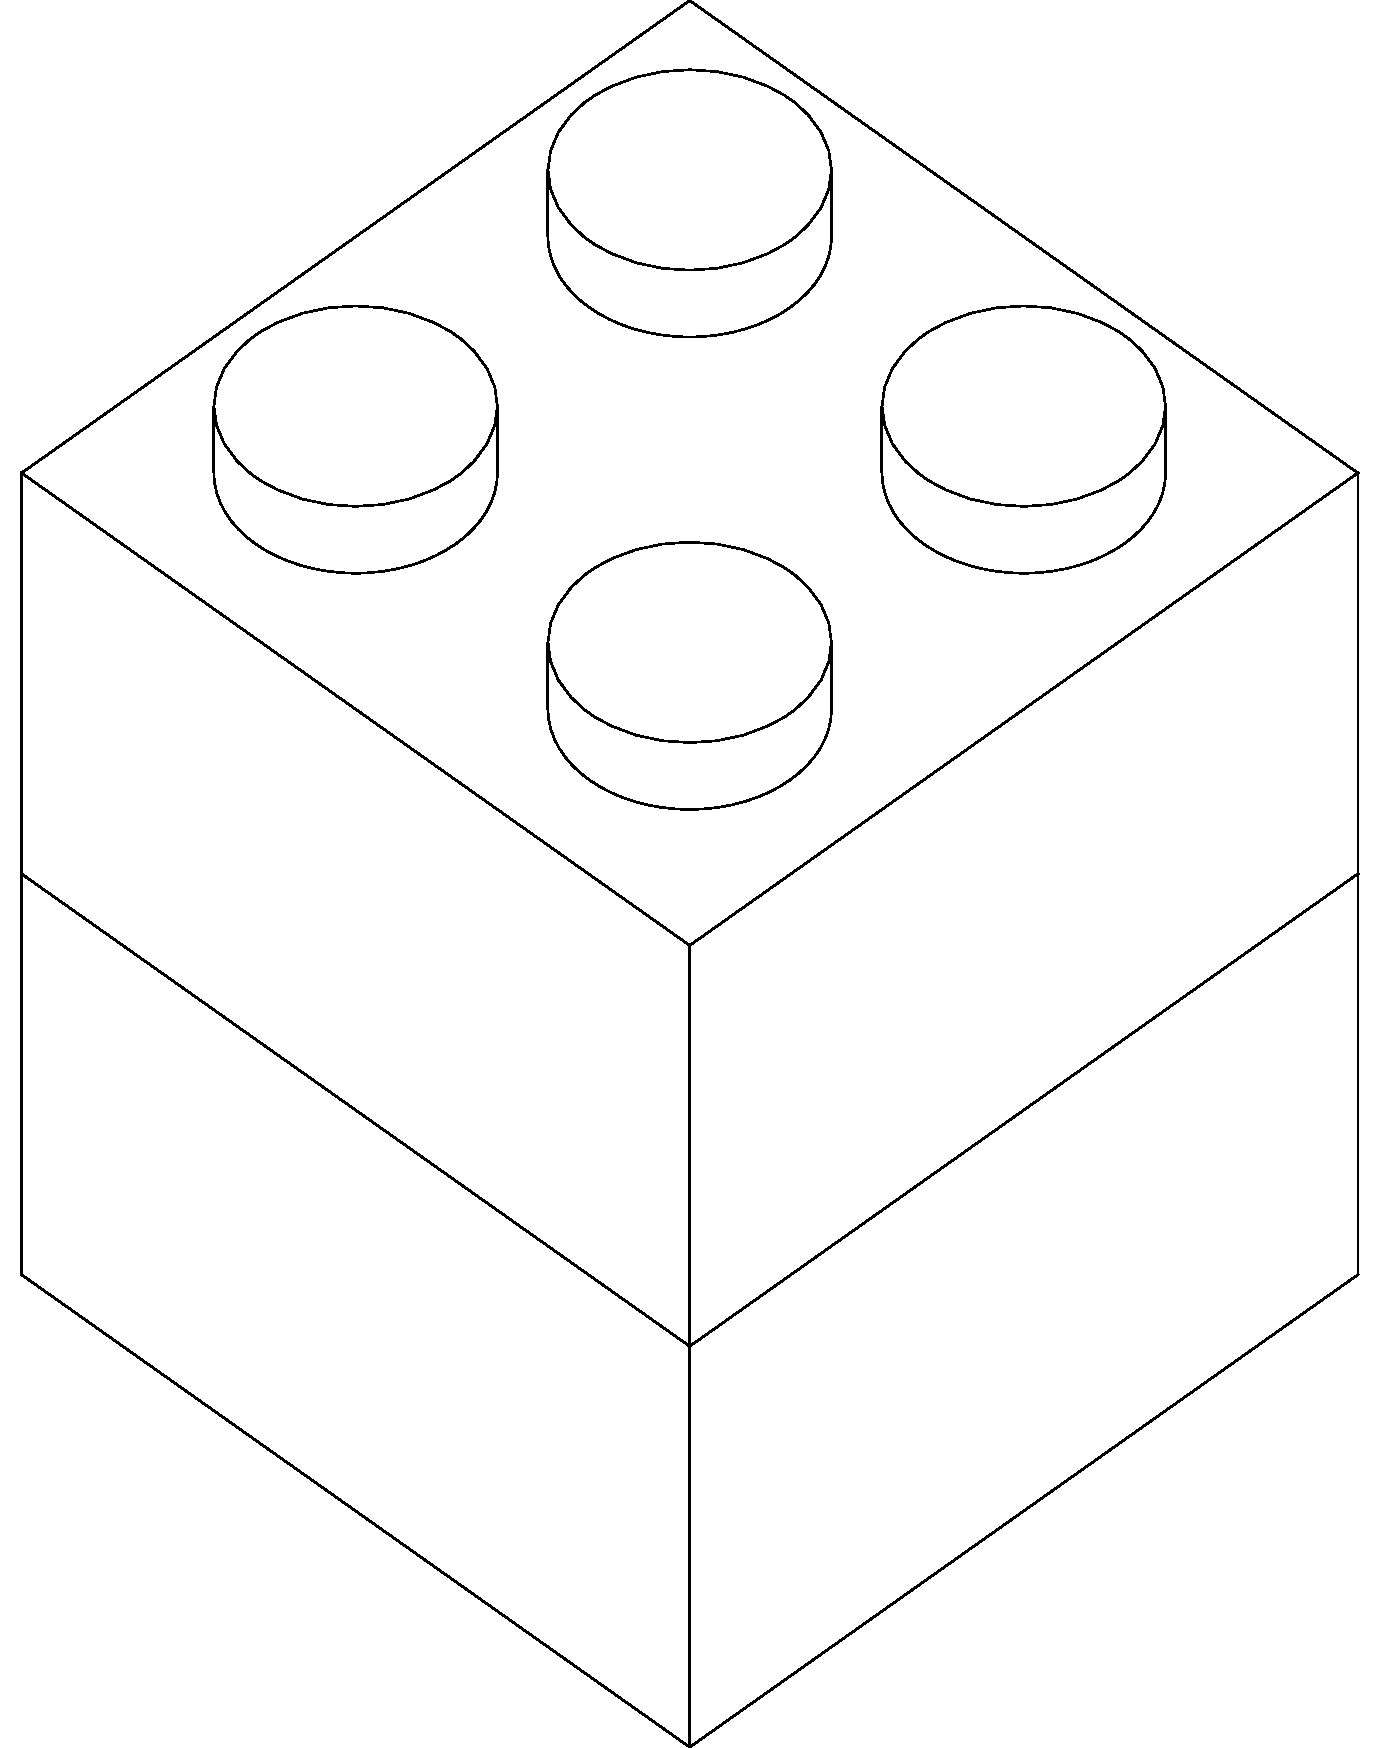
\includegraphics[width=0.09\textwidth]{figures/2x2-brick-combo-3.pdf}
        \\
        \multicolumn{1}{p{0.13\textwidth}}{
          Combination 1 Number of Pathways: 8
        } &
        \multicolumn{1}{p{0.13\textwidth}}{
          Combination 2 Number of Pathways: 8
        } &
        \multicolumn{1}{p{0.13\textwidth}}{
          Combination 3 Number of Pathways: 2
        } \\
        %Combination 1 Number of Pathways: 8 &
        %Combination 2 Number of Pathways: 8 &
        %Combination 3 Number of Pathways: 2 \\
      \end{tabular}
      \label{fig-combinations}
    \end{tikzfigure}
  }
  \block[]{References}{
    \printbibliography[heading=none]{}
  }
\end{columns}

\end{document}